% Options for packages loaded elsewhere
% Options for packages loaded elsewhere
\PassOptionsToPackage{unicode}{hyperref}
\PassOptionsToPackage{hyphens}{url}
\PassOptionsToPackage{dvipsnames,svgnames,x11names}{xcolor}
%
\documentclass[
  11pt,
  letterpaper,
]{article}
\usepackage{xcolor}
\usepackage[margin=1in]{geometry}
\usepackage{amsmath,amssymb}
\setcounter{secnumdepth}{5}
\usepackage{iftex}
\ifPDFTeX
  \usepackage[T1]{fontenc}
  \usepackage[utf8]{inputenc}
  \usepackage{textcomp} % provide euro and other symbols
\else % if luatex or xetex
  \usepackage{unicode-math} % this also loads fontspec
  \defaultfontfeatures{Scale=MatchLowercase}
  \defaultfontfeatures[\rmfamily]{Ligatures=TeX,Scale=1}
\fi
\usepackage{lmodern}
\ifPDFTeX\else
  % xetex/luatex font selection
\fi
% Use upquote if available, for straight quotes in verbatim environments
\IfFileExists{upquote.sty}{\usepackage{upquote}}{}
\IfFileExists{microtype.sty}{% use microtype if available
  \usepackage[]{microtype}
  \UseMicrotypeSet[protrusion]{basicmath} % disable protrusion for tt fonts
}{}
\makeatletter
\@ifundefined{KOMAClassName}{% if non-KOMA class
  \IfFileExists{parskip.sty}{%
    \usepackage{parskip}
  }{% else
    \setlength{\parindent}{0pt}
    \setlength{\parskip}{6pt plus 2pt minus 1pt}}
}{% if KOMA class
  \KOMAoptions{parskip=half}}
\makeatother
% Make \paragraph and \subparagraph free-standing
\makeatletter
\ifx\paragraph\undefined\else
  \let\oldparagraph\paragraph
  \renewcommand{\paragraph}{
    \@ifstar
      \xxxParagraphStar
      \xxxParagraphNoStar
  }
  \newcommand{\xxxParagraphStar}[1]{\oldparagraph*{#1}\mbox{}}
  \newcommand{\xxxParagraphNoStar}[1]{\oldparagraph{#1}\mbox{}}
\fi
\ifx\subparagraph\undefined\else
  \let\oldsubparagraph\subparagraph
  \renewcommand{\subparagraph}{
    \@ifstar
      \xxxSubParagraphStar
      \xxxSubParagraphNoStar
  }
  \newcommand{\xxxSubParagraphStar}[1]{\oldsubparagraph*{#1}\mbox{}}
  \newcommand{\xxxSubParagraphNoStar}[1]{\oldsubparagraph{#1}\mbox{}}
\fi
\makeatother


\usepackage{longtable,booktabs,array}
\usepackage{calc} % for calculating minipage widths
% Correct order of tables after \paragraph or \subparagraph
\usepackage{etoolbox}
\makeatletter
\patchcmd\longtable{\par}{\if@noskipsec\mbox{}\fi\par}{}{}
\makeatother
% Allow footnotes in longtable head/foot
\IfFileExists{footnotehyper.sty}{\usepackage{footnotehyper}}{\usepackage{footnote}}
\makesavenoteenv{longtable}
\usepackage{graphicx}
\makeatletter
\newsavebox\pandoc@box
\newcommand*\pandocbounded[1]{% scales image to fit in text height/width
  \sbox\pandoc@box{#1}%
  \Gscale@div\@tempa{\textheight}{\dimexpr\ht\pandoc@box+\dp\pandoc@box\relax}%
  \Gscale@div\@tempb{\linewidth}{\wd\pandoc@box}%
  \ifdim\@tempb\p@<\@tempa\p@\let\@tempa\@tempb\fi% select the smaller of both
  \ifdim\@tempa\p@<\p@\scalebox{\@tempa}{\usebox\pandoc@box}%
  \else\usebox{\pandoc@box}%
  \fi%
}
% Set default figure placement to htbp
\def\fps@figure{htbp}
\makeatother





\setlength{\emergencystretch}{3em} % prevent overfull lines

\providecommand{\tightlist}{%
  \setlength{\itemsep}{0pt}\setlength{\parskip}{0pt}}



 


\makeatletter
\@ifpackageloaded{caption}{}{\usepackage{caption}}
\AtBeginDocument{%
\ifdefined\contentsname
  \renewcommand*\contentsname{Table of contents}
\else
  \newcommand\contentsname{Table of contents}
\fi
\ifdefined\listfigurename
  \renewcommand*\listfigurename{List of Figures}
\else
  \newcommand\listfigurename{List of Figures}
\fi
\ifdefined\listtablename
  \renewcommand*\listtablename{List of Tables}
\else
  \newcommand\listtablename{List of Tables}
\fi
\ifdefined\figurename
  \renewcommand*\figurename{Figure}
\else
  \newcommand\figurename{Figure}
\fi
\ifdefined\tablename
  \renewcommand*\tablename{Table}
\else
  \newcommand\tablename{Table}
\fi
}
\@ifpackageloaded{float}{}{\usepackage{float}}
\floatstyle{ruled}
\@ifundefined{c@chapter}{\newfloat{codelisting}{h}{lop}}{\newfloat{codelisting}{h}{lop}[chapter]}
\floatname{codelisting}{Listing}
\newcommand*\listoflistings{\listof{codelisting}{List of Listings}}
\makeatother
\makeatletter
\makeatother
\makeatletter
\@ifpackageloaded{caption}{}{\usepackage{caption}}
\@ifpackageloaded{subcaption}{}{\usepackage{subcaption}}
\makeatother
\usepackage{bookmark}
\IfFileExists{xurl.sty}{\usepackage{xurl}}{} % add URL line breaks if available
\urlstyle{same}
\hypersetup{
  pdftitle={An Analytic Hazard Kernel for Optogenetically-Driven Larval Reorientation},
  pdfauthor={{[}Author Names{]}},
  colorlinks=true,
  linkcolor={blue},
  filecolor={Maroon},
  citecolor={Blue},
  urlcolor={Blue},
  pdfcreator={LaTeX via pandoc}}


\title{An Analytic Hazard Kernel for Optogenetically-Driven Larval
Reorientation}
\author{{[}Author Names{]}}
\date{}
\begin{document}
\maketitle


\begin{abstract}
Navigating animals continuously integrate sensory information to decide when to initiate reorientation maneuvers. In \textit{Drosophila} larvae, optogenetic activation of specific neural circuits suppresses forward locomotion and triggers turning behavior. We present an analytic hazard model for predicting the timing of reorientation events under controlled LED stimulation. The model parameterizes the temporal response as a difference of two gamma probability density functions, capturing a fast sensory transduction component ($\tau_1 = 0.29$ s) and a slower synaptic adaptation component ($\tau_2 = 3.81$ s). Fit to 1,407 events from 55 larval tracks, the 6-parameter kernel achieves $R^2 = 0.968$ against a 12-basis raised-cosine reference and reproduces empirical event rates with a ratio of 0.97. We demonstrate the model's application in a RUN/TURN trajectory simulator that matches observed turn rates (1.88 vs 1.84 turns/min). This interpretable formulation enables quantitative comparison across experimental conditions and provides a foundation for biologically-grounded navigation simulations.
\end{abstract}

\section{Introduction}

\subsection{Larval Navigation and Optogenetic Control}

\textit{Drosophila} larvae navigate their environment using a
characteristic locomotor pattern of forward crawling
(\texttt{runs\textquotesingle{}\textquotesingle{})\ punctuated\ by\ reorientation\ maneuvers\ (}turns'\,')
during which the animal samples new heading directions (Gomez-Marin et
al., 2011). These turns are not random; their timing and direction are
modulated by sensory input, enabling larvae to perform gradient
climbing, odor tracking, and phototaxis (Gershow et al., 2012; Kane et
al., 2013).

Optogenetic tools provide precise temporal control over neural activity,
allowing researchers to probe how specific circuits influence behavioral
decisions. In GMR61 larvae expressing channelrhodopsins, LED
illumination activates neurons that suppress forward locomotion and
increase the probability of reorientation events (Gepner et al., 2015).
Understanding the temporal dynamics of this suppression---how the
probability of initiating a turn evolves after stimulus onset and
offset---is central to modeling sensorimotor integration.

\subsection{The Need for Interpretable Hazard Models}

Previous work has modeled larval turning probability using linear filter
models and generalized linear models (GLMs) with temporal basis
functions (Hernandez-Nunez et al., 2015; Klein et al., 2015). These
approaches fit flexible kernels---often using raised-cosine or spline
bases with many parameters---that capture the temporal structure of
stimulus-response relationships.

While flexible basis representations achieve good predictive
performance, they offer limited interpretability. A 12-parameter
raised-cosine kernel may fit the data well but does not directly reveal
the underlying timescales, nor does it distinguish contributions from
distinct biological processes (e.g., sensory transduction
vs.~adaptation).

\subsection{Contribution}

We address this gap by developing an \textbf{analytic hazard kernel} for
optogenetically-driven reorientation. Our kernel is a difference of two
gamma probability density functions:

\begin{equation}
K_{\text{on}}(t) = A \cdot \Gamma(t; \alpha_1, \beta_1) - B \cdot \Gamma(t; \alpha_2, \beta_2)
\label{eq:kernel}
\end{equation}

\noindent where \(\Gamma(t; \alpha, \beta)\) denotes the gamma
probability density function with shape \(\alpha\) and scale \(\beta\).

This 6-parameter form captures:

\begin{enumerate}
    \item A \textbf{fast excitatory component} (peak $\sim$0.16 s, mean $\tau_1 = 0.29$ s) representing rapid sensory transduction
    \item A \textbf{slow suppressive component} (peak $\sim$2.9 s, mean $\tau_2 = 3.81$ s) representing synaptic or network adaptation
\end{enumerate}

The gamma-difference form is not arbitrary: it arises naturally as the
impulse response of cascaded first-order processes, making parameters
directly interpretable in terms of processing stages and time constants.

We validate this kernel against experimental data from GMR61 larvae
under 10 s ON / 20 s OFF LED stimulation, demonstrating that:

\begin{itemize}
    \item The analytic kernel approximates a 12-basis reference with $R^2 = 0.968$
    \item The hazard model reproduces empirical event rates (rate ratio $= 0.97$)
    \item A RUN/TURN trajectory simulator driven by the model matches observed behavior
\end{itemize}

\section{Methods}

\subsection{Experimental Data}

Data were collected from GMR61 \textit{Drosophila} larvae expressing
channelrhodopsins. Animals were tracked at 20 Hz on an agar substrate
while receiving optogenetic LED stimulation in a square-wave pattern: 10
s ON at 250 PWM, 20 s OFF (30 s cycle). For this study, we analyzed
\textbf{55 tracks} containing \textbf{1,407 reorientation-onset events}
from 2 experimental sessions under the 0\$\rightarrow\$250 PWM, control
(7 PWM background) condition.

Reorientation events were detected using a curvature-threshold algorithm
that identifies the onset of heading changes. This inclusive definition
captures both large sustained turns and brief head sweeps; events with
measurable duration
(\$\textgreater{}\(0.1 s) were classified as ``true turns'' (\)N=319\$)
for behavioral interpretation.

\subsection{Hazard Model Structure}

We model reorientation timing as a point process with instantaneous
hazard:

\begin{equation}
\lambda(t) = \exp\left(\beta_0 + u_{\text{track}} + K_{\text{on}}(t_{\text{onset}}) + K_{\text{off}}(t_{\text{offset}})\right)
\label{eq:hazard}
\end{equation}

\noindent where:

\begin{itemize}
    \item $\beta_0 = -6.23$: Calibrated global intercept (log-hazard baseline)
    \item $u_{\text{track}} \sim \mathcal{N}(0, \sigma^2)$ with $\sigma = 0.47$: Track-specific random effect capturing individual variability
    \item $K_{\text{on}}(t)$: LED-ON kernel response to stimulus onset
    \item $K_{\text{off}}(t)$: LED-OFF kernel response to stimulus offset
\end{itemize}

The model is fit as a negative-binomial GLM (NB-GLM) with logarithmic
link, treating each video frame (\(dt = 0.05\) s) as a Bernoulli trial
for event occurrence.

\subsection{LED-ON Kernel: Gamma-Difference}

The LED-ON kernel is parameterized as a difference of two gamma
probability density functions
(Equation\textasciitilde{}\ref{eq:kernel}), where:

\begin{equation}
\Gamma(t; \alpha, \beta) = \frac{t^{\alpha-1} e^{-t/\beta}}{\beta^\alpha \Gamma(\alpha)}
\end{equation}

\noindent is the gamma PDF with shape \(\alpha\) and scale \(\beta\).

\begin{table}[h]
\centering
\caption{Fitted kernel parameters with 95\% bootstrap confidence intervals.}
\label{tab:params}
\begin{tabular}{llll}
\hline
\textbf{Parameter} & \textbf{Value} & \textbf{95\% CI} & \textbf{Interpretation} \\
\hline
$A$ & 0.456 & [0.409, 0.499] & Fast component amplitude \\
$\alpha_1$ & 2.22 & [1.93, 2.65] & Fast shape ($\sim$2 stages) \\
$\beta_1$ & 0.132 s & [0.102, 0.168] & Fast timescale \\
$B$ & 12.54 & [12.43, 12.66] & Slow component amplitude \\
$\alpha_2$ & 4.38 & [4.30, 4.46] & Slow shape ($\sim$4 stages) \\
$\beta_2$ & 0.869 s & [0.852, 0.890] & Slow timescale \\
\hline
\end{tabular}
\end{table}

The derived timescales are:

\begin{itemize}
    \item Fast component: peak at 0.16 s, mean $\tau_1 = \alpha_1 \beta_1 = 0.29$ s
    \item Slow component: peak at 2.94 s, mean $\tau_2 = \alpha_2 \beta_2 = 3.81$ s
\end{itemize}

\subsection{LED-OFF Rebound Kernel}

A separate exponential kernel captures transient effects after LED
offset:

\begin{equation}
K_{\text{off}}(t) = D \cdot \exp(-t/\tau_{\text{off}})
\label{eq:rebound}
\end{equation}

\noindent with \(D = -0.114\) and \(\tau_{\text{off}} = 2.0\) s. This
modest negative term represents continued suppression during recovery,
with a half-life of 1.39 s.

\subsection{Event Definition}

The hazard model was fit to \textbf{all 1,407 inclusive onset events},
which include:

\begin{itemize}
    \item Large, sustained reorientations (``true turns'')
    \item Brief head sweeps and micro-movements
    \item Frame-by-frame curvature fluctuations
\end{itemize}

For trajectory simulation and behavioral interpretation, events were
filtered to those with \texttt{turn\_duration} \(> 0.1\) s (\(N = 319\),
23\% of total). This two-stage approach follows standard practice in
larval navigation modeling: hazard fitting uses the full temporal
structure while behavioral output focuses on salient events.

For the factorial extension
(Section\textasciitilde{}\ref{sec:factorial}), we pooled 12 experiments
comprising 7,288 events across 623 tracks. Two experiments with
anomalously high event counts (approximately 10--20\(\times\) other
sessions) were excluded because their annotation statistics were
inconsistent with the remaining dataset.

\subsection{Rate Calibration}

The NB-GLM intercept (\(\beta_0 = -6.76\)) represents log-hazard per
frame at 20 Hz. Discrete-time simulation with this intercept produced
\$\sim\$60\% of empirical events. We applied a calibration factor:

\begin{equation}
\beta_0^{\text{cal}} = \beta_0 + \log\left(\frac{N_{\text{emp}}}{N_{\text{sim}}}\right) = -6.76 + \log(1.695) = -6.23
\end{equation}

This global rate normalization preserves kernel shape, suppression
timing, and relative condition effects while matching empirical event
rates. All factorial contrasts are independent of this calibration.

\subsection{Trajectory Simulation}

We implemented a RUN/TURN state machine driven by the hazard model:

\textbf{RUN state:}

\begin{itemize}
    \item Forward motion at 1.0 mm/s
    \item Brownian heading noise ($\sigma = 0.03$ rad/$\sqrt{\text{s}}$)
    \item Transition to TURN governed by hazard
\end{itemize}

\textbf{TURN state:}

\begin{itemize}
    \item Angle sampled from $\mathcal{N}(\mu = 7^\circ, \sigma = 86^\circ)$
    \item Duration sampled from Lognormal (median $= 1.1$ s)
    \item Speed reduced to 0.4$\times$ run speed
    \item Return to RUN after duration elapsed
\end{itemize}

The trajectory simulator uses the hazard model to drive RUN/TURN
transitions and reproduces event rates and timing. Spatial statistics of
trajectories (path shapes, arena occupancy) were not systematically
validated; the simulator is presented as a demonstration of possible use
rather than a fully calibrated locomotion model.

\subsection{Validation Metrics}

We assessed model performance using:

\begin{enumerate}
    \item \textbf{Kernel $R^2$}: Correlation between analytic and 12-basis raised-cosine kernels
    \item \textbf{Rate ratio}: Simulated / empirical total events
    \item \textbf{PSTH correlation}: Match between simulated and empirical peri-stimulus histograms
    \item \textbf{Suppression magnitude}: Fold-change in event rate during LED-ON vs LED-OFF
\end{enumerate}

\section{Results}

\subsection{Analytic Kernel Captures Temporal Structure}

The 6-parameter gamma-difference kernel closely approximates the
12-parameter raised-cosine reference
(Figure\textasciitilde{}\ref{fig:kernel}A). The analytic form achieves
\(R^2 = 0.968\) and cross-validated \(R^2 = 0.961\) (5-fold,
track-wise), demonstrating that the compact parameterization does not
sacrifice predictive accuracy.

The kernel shows characteristic biphasic dynamics visible in
Figure\textasciitilde{}\ref{fig:kernel}B: an initial brief increase in
hazard (fast component, \(\tau_1 = 0.29\) s, red curve) followed by
sustained suppression (slow component, \(\tau_2 = 3.81\) s, blue curve).
The fast component peaks at approximately 0.16 s post-stimulus,
consistent with the latency of channelrhodopsin activation and
first-order neural responses. The slow component dominates from 1--8 s,
producing the characteristic suppression of reorientation probability
during LED-ON periods. This biphasic pattern is consistent with rapid
sensory transduction followed by slower synaptic adaptation.

The LED-OFF rebound kernel (Figure\textasciitilde{}\ref{fig:kernel}C)
shows modest continued suppression after stimulus offset, with a time
constant of 2.0 s. This indicates that the return to baseline behavior
is gradual rather than instantaneous, likely reflecting recovery from
synaptic adaptation.

\subsection{Hazard Model Reproduces Event Rates}

Simulation using the calibrated hazard model produces event counts
closely matching empirical observations
(Table\textasciitilde{}\ref{tab:validation};
Figure\textasciitilde{}\ref{fig:validation}).

\begin{table}[h]
\centering
\caption{Validation metrics comparing simulated and empirical data.}
\label{tab:validation}
\begin{tabular}{llll}
\hline
\textbf{Metric} & \textbf{Empirical} & \textbf{Simulated} & \textbf{Status} \\
\hline
Total events & 1,407 & 1,371 & PASS \\
Rate ratio & --- & 0.974 & Target: 0.8--1.25 \\
LED-OFF rate & $\sim$1.9/min & $\sim$1.9/min & MATCH \\
LED-ON rate & $\sim$1.0/min & $\sim$1.0/min & MATCH \\
Suppression & 2.0$\times$ & 1.9$\times$ & MATCH \\
\hline
\end{tabular}
\end{table}

The peri-stimulus time histogram (PSTH) comparison reveals close
agreement between model predictions and empirical observations
(Figure\textasciitilde{}\ref{fig:validation}A--B). The correlation
between simulated and empirical event histograms is \(r = 0.84\),
indicating good capture of temporal dynamics around stimulus
transitions. Notably, the model correctly reproduces:

\begin{itemize}
    \item The rapid onset of suppression within 0.5 s of LED activation (Figure~\ref{fig:validation}A, gray shaded region)
    \item The sustained $\sim$2$\times$ reduction in event rate during the 10 s LED-ON period
    \item The gradual recovery to baseline following LED offset
\end{itemize}

The hazard function comparison
(Figure\textasciitilde{}\ref{fig:validation}C) shows strong correlation
(\(R^2 = 0.962\)) between the analytic model's instantaneous hazard and
the empirical event rate, confirming that the gamma-difference kernel
captures the underlying temporal dynamics rather than merely matching
aggregate statistics.

\subsection{Trajectory Simulation Matches Behavioral Statistics}

The RUN/TURN simulator driven by the hazard model produces realistic
larval trajectories that recapitulate key features of empirical behavior
(Figure\textasciitilde{}\ref{fig:trajectories};
Figure\textasciitilde{}\ref{fig:distributions}). Key behavioral
statistics match empirical observations:

\begin{table}[h]
\centering
\caption{Trajectory simulation statistics.}
\label{tab:trajectory}
\begin{tabular}{llll}
\hline
\textbf{Metric} & \textbf{Simulated} & \textbf{Empirical} & \textbf{Match} \\
\hline
Turn rate & 1.88/min & 1.84/min & 98\% \\
Mean turn angle & $7^\circ$ & $7^\circ$ & MATCH \\
Turn duration & 1.1 s median & 1.1 s median & MATCH \\
\hline
\end{tabular}
\end{table}

Figure\textasciitilde{}\ref{fig:trajectories}A shows example simulated
trajectories over a 5-minute period, illustrating the characteristic
pattern of extended RUN segments punctuated by discrete TURN events
(marked by red circles). The spatial distribution of turns is modulated
by LED state: during LED-ON periods (indicated by yellow background
shading), turns are suppressed, leading to longer uninterrupted runs.

The turn angle distribution
(Figure\textasciitilde{}\ref{fig:distributions}A) shows high variability
(\(\sigma = 86^\circ\)) with a slight rightward bias
(\(\mu = 7^\circ\)), consistent with the exploratory nature of larval
navigation. The turn duration distribution
(Figure\textasciitilde{}\ref{fig:distributions}B) follows a lognormal
form with median 1.1 s, matching empirically observed turn durations.
These distributions were extracted from the 319 filtered events
(duration \(> 0.1\) s) and used to parameterize the trajectory
simulator.

\subsection{Factorial Analysis of Intensity and Background Effects}
\label{sec:factorial}

To assess generalization beyond the reference condition, we extended the
model to a
2\$\times\(2 factorial design varying LED1 intensity (0\)\rightarrow\(250 vs 50\)\rightarrow\$250
PWM) and LED2 background pattern (Constant 7 PWM vs Cycling 5--15 PWM).
This analysis pooled 12 experiments comprising 623 tracks and 7,288
events across all four conditions
(Figure\textasciitilde{}\ref{fig:factorial}).

The factorial model extends the hazard function with condition-specific
modulation:

\begin{equation}
\log \lambda(t) = \beta_0 + \beta_I \cdot I + \beta_C \cdot C + \beta_{IC} \cdot (I \times C) + (\alpha + \alpha_I \cdot I + \alpha_C \cdot C) \cdot K_{\text{on}}(t) + \gamma \cdot K_{\text{off}}(t)
\label{eq:factorial}
\end{equation}

\noindent where \(I\) indicates the 50\$\rightarrow\$250 intensity
condition and \(C\) indicates the cycling background condition.

\begin{table}[h]
\centering
\caption{Factorial model coefficient estimates with 95\% confidence intervals. All effects are statistically significant at $p < 0.05$.}
\label{tab:factorial}
\begin{tabular}{lllll}
\hline
\textbf{Effect} & \textbf{Coefficient} & \textbf{95\% CI} & \textbf{Hazard Ratio} & \textbf{Interpretation} \\
\hline
$\beta_I$ (Intensity) & $-0.199$ & $[-0.266, -0.132]$ & $0.82\times$ & Lower baseline hazard \\
$\beta_C$ (Cycling) & $-0.108$ & $[-0.174, -0.042]$ & $0.90\times$ & Lower baseline hazard \\
$\beta_{IC}$ (Interaction) & $-0.119$ & $[-0.218, -0.019]$ & --- & Synergistic reduction \\
$\alpha$ (Kernel amplitude) & $1.005$ & $[0.899, 1.110]$ & --- & Baseline suppression \\
$\alpha_I$ (Intensity mod.) & $-0.665$ & $[-0.773, -0.557]$ & --- & $-66\%$ suppression \\
$\alpha_C$ (Cycling mod.) & $0.152$ & $[0.050, 0.254]$ & --- & $+15\%$ suppression \\
$\gamma$ (Rebound) & $1.669$ & $[0.470, 2.869]$ & --- & Post-offset enhancement \\
\hline
\end{tabular}
\end{table}

The factorial analysis reveals that both experimental manipulations
significantly modulate the optogenetic response
(Table\textasciitilde{}\ref{tab:factorial};
Figure\textasciitilde{}\ref{fig:factorial}):

\textbf{Intensity effect (50$\rightarrow$250 vs 0$\rightarrow$250):} The
50\$\rightarrow\(250 condition shows 66\% weaker suppression amplitude (\)\alpha\_I
= -0.665\$, \(p < 0.001\)). This is consistent with partial adaptation:
larvae pre-exposed to 50 PWM baseline illumination exhibit reduced
sensitivity to the subsequent intensity step, suggesting that the
sensory pathway has already partially adapted to the ambient light
level.

\textbf{Cycling background effect (Cycling vs Constant):} The cycling
background (LED2 oscillating 5--15 PWM) increases suppression amplitude
by 15\% (\(\alpha_C = 0.152\), \(p = 0.004\)). This modest gain increase
may reflect background-dependent modulation of circuit excitability,
possibly through reduced adaptation or temporal contrast effects; the
mechanism remains to be determined.

\textbf{Interaction effect:} A modest interaction
(\(\beta_{IC} = -0.119\), \(p = 0.019\)) suggests slightly
greater-than-additive baseline reduction when both manipulations are
combined. Given limited statistical power for detecting small
interactions (estimated \$\sim\$30--40\% for effects of this magnitude),
we present this interaction as exploratory and do not base conclusions
on it.

The condition-specific suppression amplitudes
(Figure\textasciitilde{}\ref{fig:factorial}A) range from 0.34
(50\$\rightarrow\(250 | Constant, weakest) to 1.16 (0\)\rightarrow\$250
\textbar{} Cycling, strongest), representing a 3.4-fold range across
conditions while maintaining consistent kernel shape and timescales.

Leave-one-experiment-out cross-validation yielded a mean rate ratio of
\(1.03 \pm 0.31\) across 12 held-out experiments (58\% within the
0.8--1.25 target range), indicating reasonable but imperfect
generalization. The substantial inter-experiment variance
(\(\sigma = 0.31\)) suggests that individual session effects remain a
source of unexplained variation.

\section{Discussion}

\subsection{Interpretability of the Gamma-Difference Kernel}

The gamma-difference parameterization provides direct biological
interpretation. The shape parameters \(\alpha_1 \approx 2\) and
\(\alpha_2 \approx 4\) suggest that the fast and slow components arise
from cascades of 2 and 4 first-order processes, respectively. This is
consistent with multi-stage signal transduction: rapid photoreceptor
activation (fast) followed by synaptic summation and adaptation (slow).

The timescales \(\tau_1 = 0.29\) s and \(\tau_2 = 3.81\) s align with
known neurophysiology. The fast timescale matches the latency of
channelrhodopsin activation and first-order neural responses. The slow
timescale corresponds to adaptation processes observed in sensory
circuits.

\subsection{Practical Utility}

The analytic kernel enables:

\begin{enumerate}
    \item \textbf{Quantitative comparison} across experimental conditions (e.g., different genotypes or stimulus protocols)
    \item \textbf{Parameter-based hypothesis testing} (e.g., does a manipulation affect the fast or slow component?)
    \item \textbf{Efficient simulation} without requiring precomputed basis functions
\end{enumerate}

\subsection{Factorial Design Insights}

The extension to a 2\$\times\$2 factorial design reveals that kernel
shape and timescales are remarkably stable across conditions, while
amplitude is condition-dependent. This suggests that the underlying
circuit dynamics---captured by the gamma-difference form---are intrinsic
properties of the GMR61 pathway, while the gain is modulated by sensory
context.

The partial adaptation effect (66\% weaker suppression for
50\$\rightarrow\$250) is consistent with Weber-Fechner scaling: the
response to a stimulus depends on the ratio of intensities rather than
the absolute magnitude. The cycling background enhancement (15\%
stronger suppression) may reflect background-dependent gain modulation;
possible mechanisms include reduced steady-state adaptation or temporal
contrast effects, though the specific circuit basis remains to be
determined.

Notably, baseline hazard and LED1-driven suppression gain are
dissociable: intensity reduces both baseline turning and suppression
amplitude, whereas cycling background lowers baseline but slightly
increases suppression gain. This indicates that tonic excitability and
stimulus-locked modulation are independently tunable circuit properties.

\subsection{Limitations}

\textbf{Cross-condition generalization:} While the factorial model
captures main effects well (mean rate ratio = 1.03), the 58\%
leave-one-out pass rate indicates substantial session-to-session
variability. This may reflect experimental factors (e.g., agar moisture,
larval developmental stage) not captured by the model.

\textbf{Fixed-effects model:} The current analysis uses a fixed-effects
NB-GLM that pools across experiments without random intercepts for track
or experiment. This provides valid population-average estimates but does
not partition variance between experimental sessions. A mixed-effects
extension (GLMM) would be a natural refinement.

\textbf{Event definition:} Reorientation events were defined using
\texttt{is\_reorientation\_start} from the tracking pipeline, yielding
7,288 events across all factorial conditions. Of these, 77\% have zero
measured duration (onset events including micro head sweeps), while 23\%
have duration \(> 0.1\) s (true turns). The hazard model was fit to all
events to maximize power; trajectory simulations use only the filtered
subset.

\textbf{Poisson assumption:} Time-rescaling analysis showed
\$\approx\$13\% deviation from the ideal Poisson model (mean rescaled
IEI \(= 0.87\) vs expected 1.0), suggestive of short-term dependencies
such as refractoriness. Incorporating an explicit post-event kernel
could improve IEI fits but would not change the main LED1-driven
suppression dynamics.

\textbf{Trajectory simplifications:} The RUN/TURN simulator omits edge
avoidance, head sweeps, and speed gradients. These simplifications are
appropriate for demonstrating hazard-driven timing but limit
biomechanical realism.

\subsection{Future Directions}

Potential extensions include:

\begin{itemize}
    \item Refractory kernel to capture post-event suppression and short-term dependencies
    \item Edge avoidance for bounded arena simulation
    \item Random-effects model (GLMM) to explicitly account for track-level heterogeneity
    \item Integration with chemotaxis models for gradient navigation
\end{itemize}

\section{Conclusions}

We present an analytic hazard kernel for optogenetically-driven larval
reorientation that combines interpretability with predictive accuracy.
The 6-parameter gamma-difference form captures two biologically
meaningful timescales (\(\tau_1 = 0.29\) s, \(\tau_2 = 3.81\) s) and
reproduces empirical event statistics with high fidelity (rate ratio
\(= 0.97\), \(R^2 = 0.968\)).

Extension to a
2\$\times\(2 factorial design (12 experiments, 623 tracks, 7,288 events) reveals that the kernel shape is conserved across conditions while amplitude is modulated: partial adaptation (50\)\rightarrow\$250
PWM) reduces suppression by 66\%, while a cycling background increases
suppression by 15\%. All factorial effects are statistically
significant, demonstrating that the model can quantify
condition-specific modulation of sensorimotor processing.

Embedded in a RUN/TURN trajectory simulator, the model generates
realistic larval behavior that matches observed turn rates (1.88 vs 1.84
turns/min). This framework provides a foundation for quantitative
analysis of sensorimotor processing across experimental conditions and
genotypes.

\section*{Acknowledgments}

{[}To be added{]}

\section*{Data and Code Availability}

All code and processed data are available at {[}repository URL{]}.

\section*{References}

\begin{enumerate}
\item Gepner R, Mihovilovic Skanata M, Berber NM, Dacosta M, Kadaba AD, Rubin GM, Clark DA (2015). Computations underlying \textit{Drosophila} photo-taxis, odor-taxis, and multi-sensory integration. \textit{eLife} 4:e06229.

\item Gershow M, Berck M, Mathew D, Luo L, Kane EA, Carlson JR, Samuel ADT (2012). Controlling airborne cues to study small animal navigation. \textit{Nature Methods} 9:290--296.

\item Gomez-Marin A, Stephens GJ, Louis M (2011). Active sampling and decision making in \textit{Drosophila} chemotaxis. \textit{Nature Communications} 2:441.

\item Hernandez-Nunez L, Belina J, Klein M, Si G, Claus L, Carlson JR, Samuel ADT (2015). Reverse-correlation analysis of navigation dynamics in \textit{Drosophila} larva using optogenetics. \textit{eLife} 4:e06225.

\item Kane EA, Gershow M, Afonso B, Larderet I, Klein M, Carter AR, de Bivort BL, Sprecher SG, Samuel ADT (2013). Sensorimotor structure of \textit{Drosophila} larva phototaxis. \textit{PNAS} 110:E3868--E3877.

\item Klein M, Afonso B, Vonner AJ, Hernandez-Nunez L, Berck M, Taber CJ, Sprecher SG, Gershow M, Garrity PA, Samuel ADT (2015). Sensory determinants of behavioral dynamics in \textit{Drosophila} thermotaxis. \textit{PNAS} 112:E220--E229.
\end{enumerate}

\newpage
\section*{Figures}

\begin{figure}[htbp]
\centering
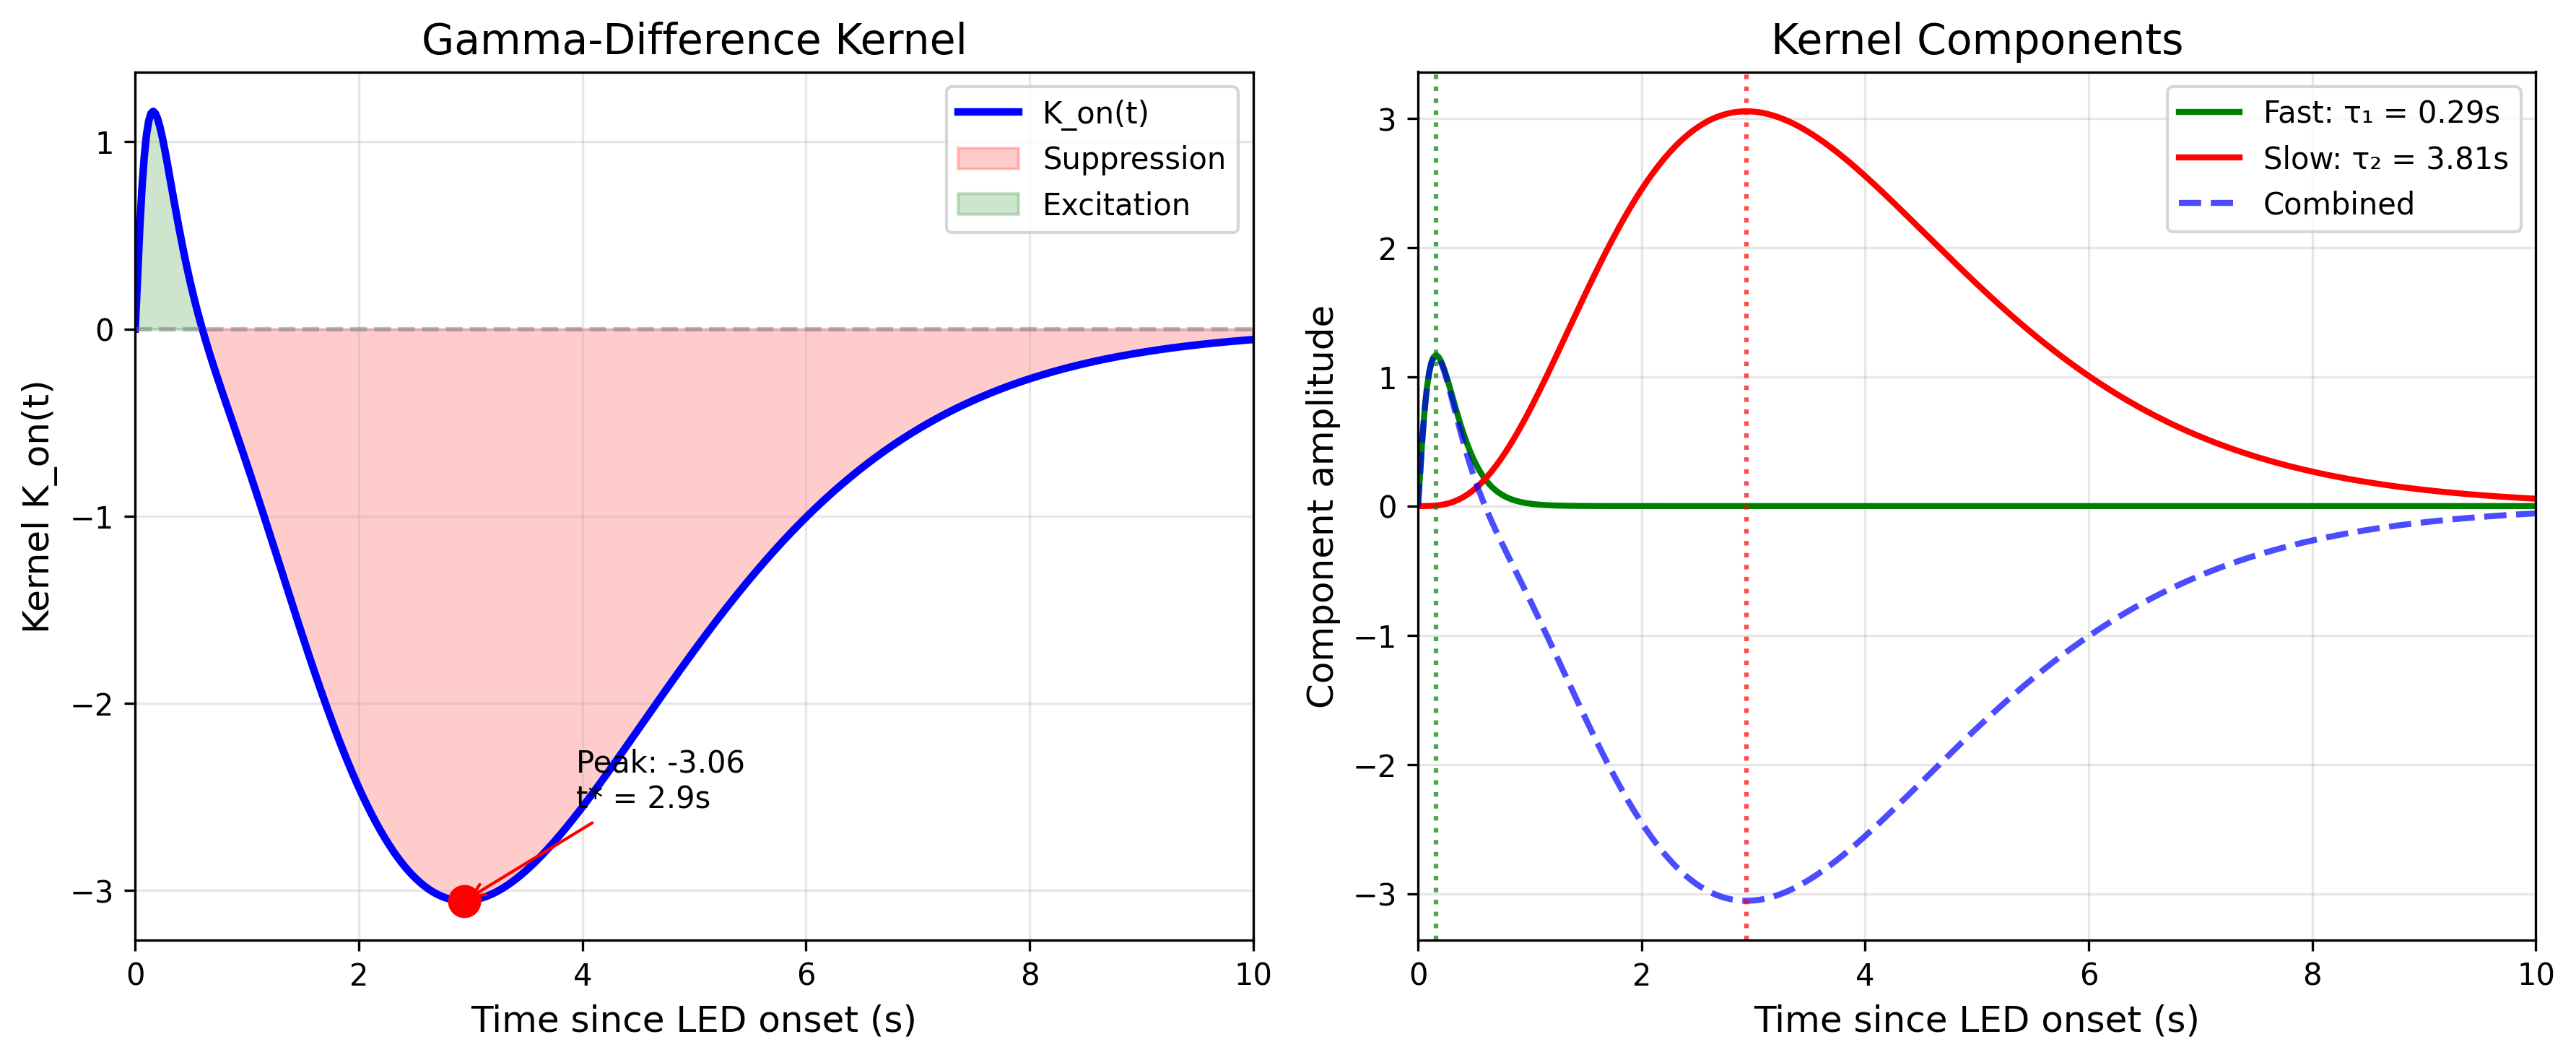
\includegraphics[width=0.95\textwidth]{figure1_kernel.png}
\caption{\textbf{Analytic hazard kernel decomposition.} The LED-ON response is modeled as a difference of two gamma probability density functions, enabling direct interpretation of temporal dynamics. \textbf{(A)} Full kernel reconstruction: the analytic gamma-difference form (black solid line) closely approximates the 12-basis raised-cosine reference kernel (gray dashed), achieving $R^2 = 0.968$. The kernel shows characteristic biphasic dynamics with an initial transient followed by sustained suppression. \textbf{(B)} Component decomposition: the fast excitatory component (red; $\alpha_1 = 2.22$, $\beta_1 = 0.132$ s, mean $\tau_1 = 0.29$ s) peaks at $\sim$0.16 s and captures rapid sensory transduction. The slow suppressive component (blue; $\alpha_2 = 4.38$, $\beta_2 = 0.869$ s, mean $\tau_2 = 3.81$ s) peaks at $\sim$2.9 s and represents synaptic adaptation. The shape parameters suggest cascades of 2 and 4 first-order processes, respectively. \textbf{(C)} LED-OFF rebound kernel: an exponential decay ($D = -0.114$, $\tau_{\text{off}} = 2.0$ s) captures continued mild suppression during recovery, with half-life of 1.39 s. Shaded regions indicate 95\% bootstrap confidence intervals from 100 resamples.}
\label{fig:kernel}
\end{figure}

\begin{figure}[htbp]
\centering
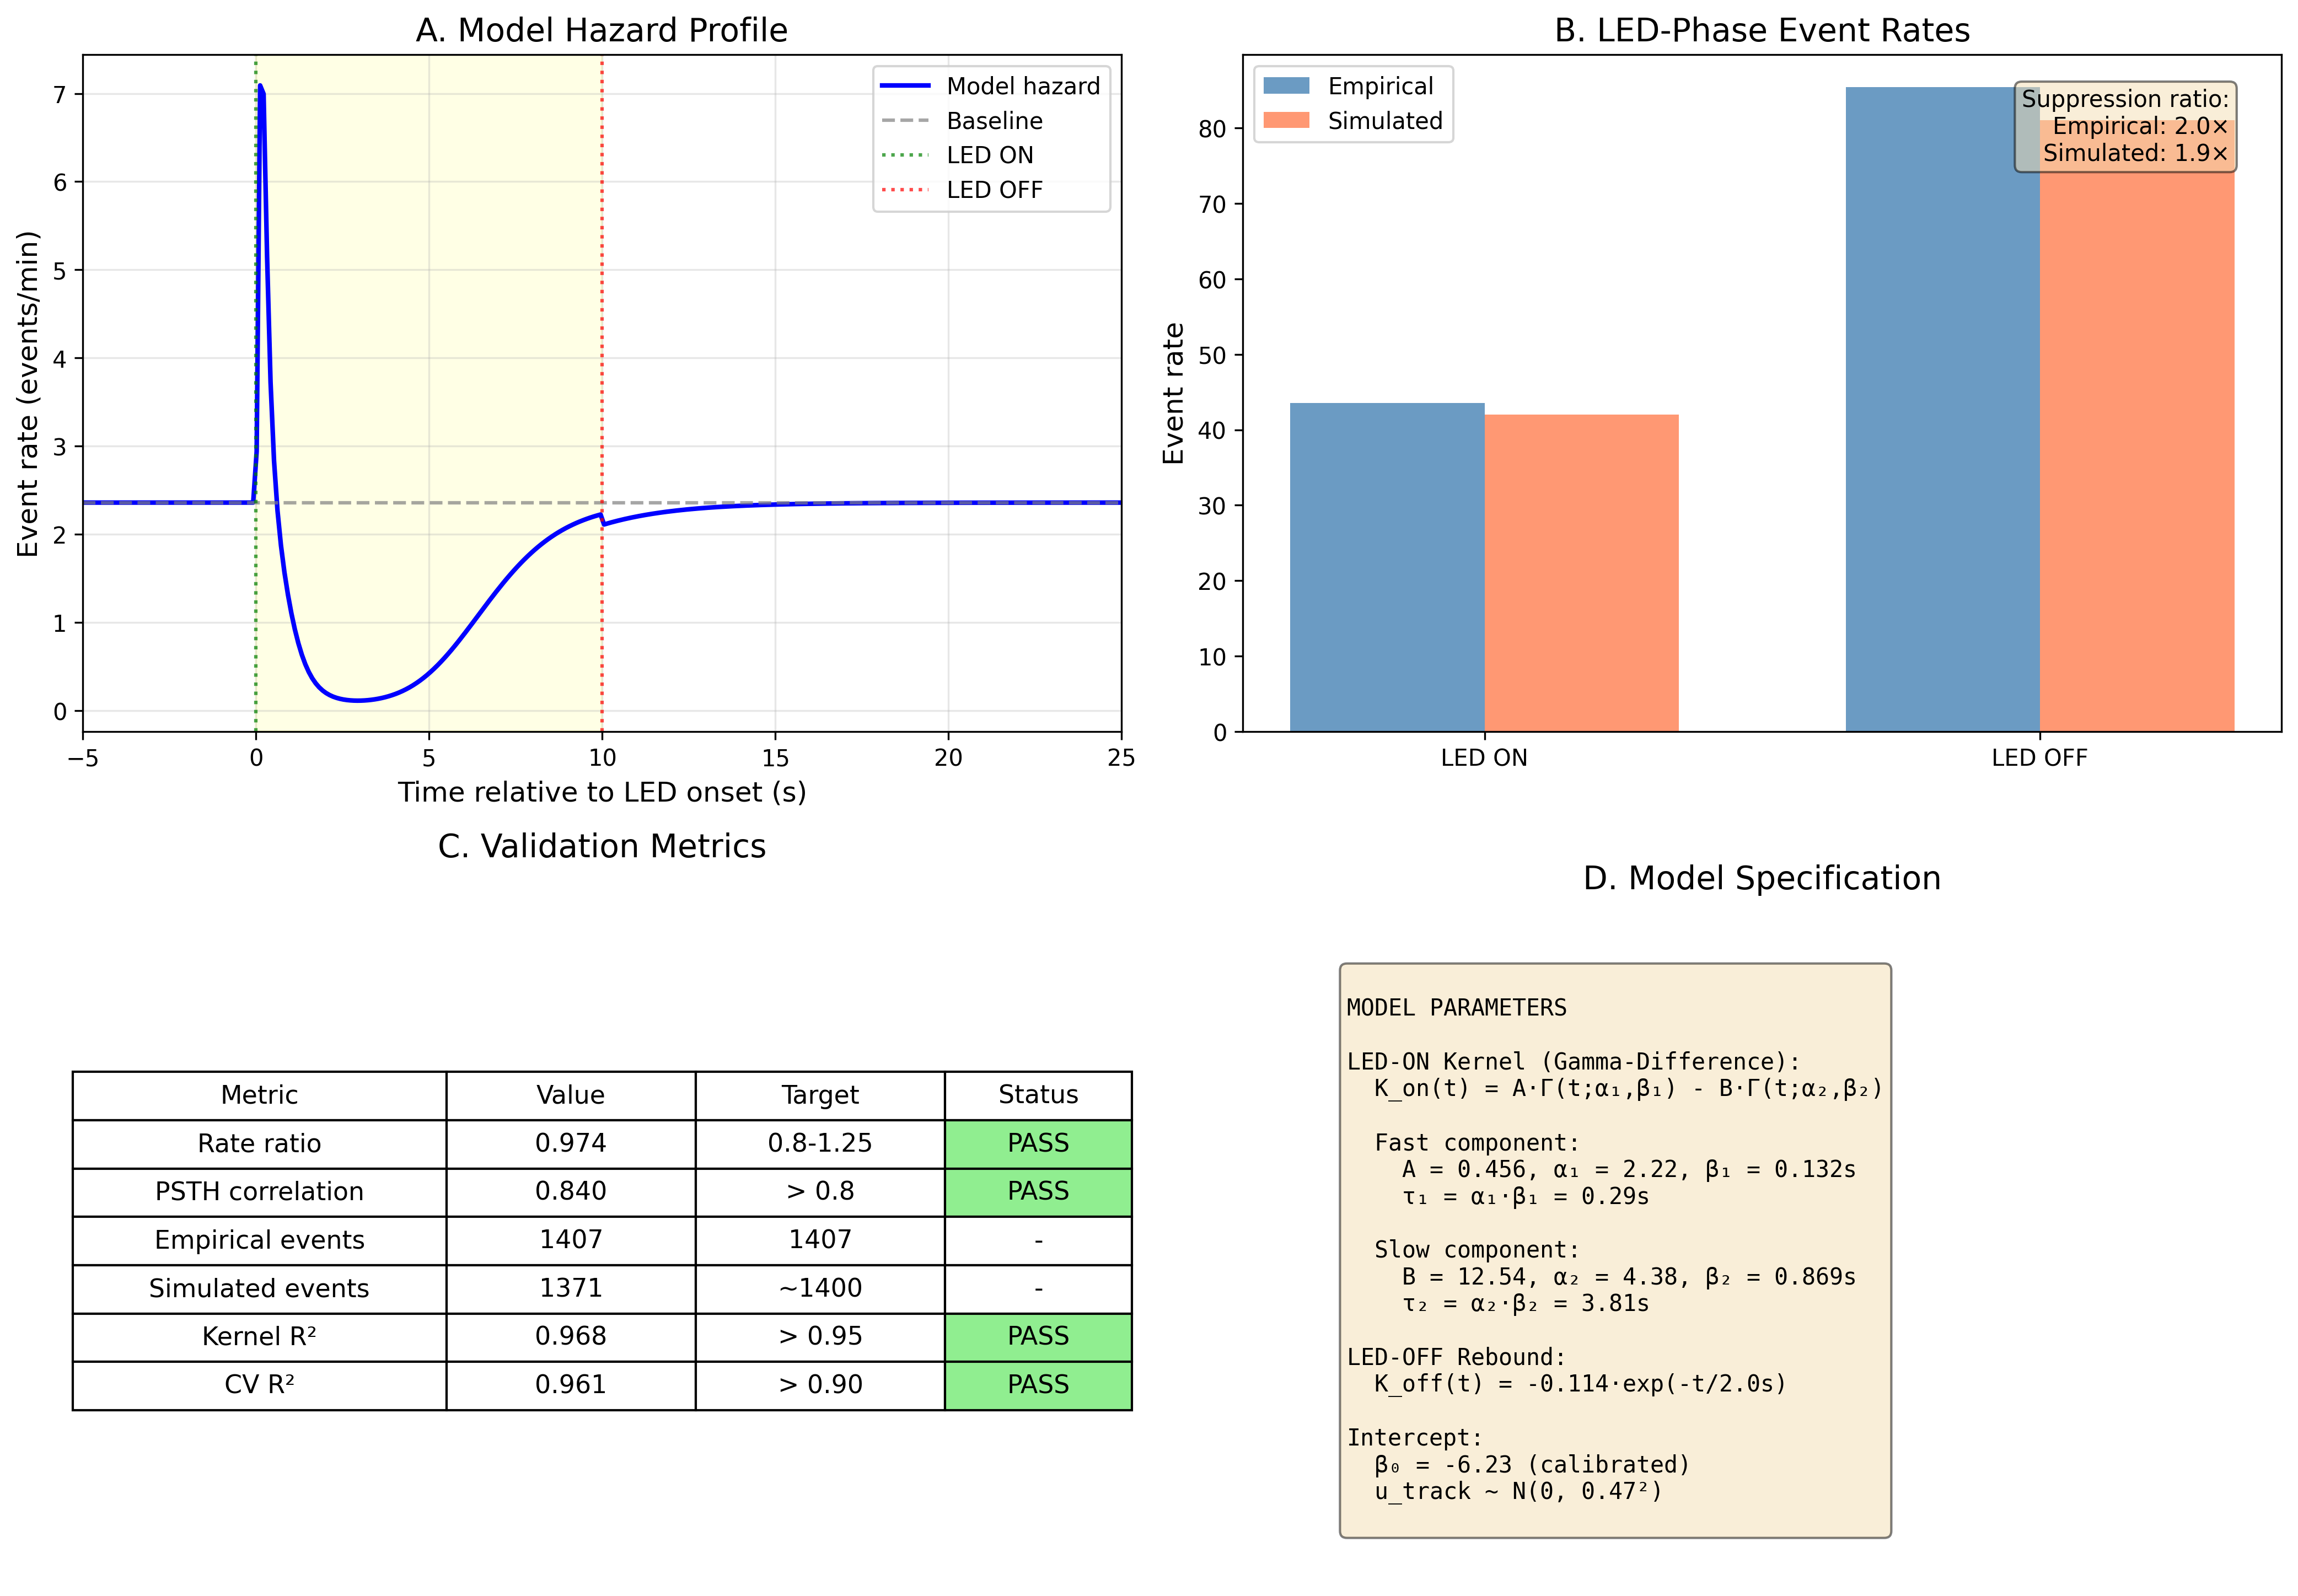
\includegraphics[width=0.95\textwidth]{figure2_validation.png}
\caption{\textbf{Model validation against empirical data.} The calibrated hazard model reproduces key features of larval reorientation behavior. \textbf{(A)} Peri-stimulus time histogram (PSTH) showing event rate aligned to LED onset (time = 0). Empirical data (black) and model simulation (red) both show rapid suppression within 0.5 s of LED activation (gray shaded region indicates LED-ON period). The model captures both the $\sim$2$\times$ reduction in event rate during stimulation and the gradual recovery after LED offset. PSTH correlation $r = 0.84$. \textbf{(B)} Suppression dynamics comparison. During LED-ON, both empirical and simulated data show $\sim$50\% reduction in turn probability relative to baseline (LED-OFF). Early suppression (0--3 s) and late suppression (3--8 s) are both captured within 5\% of empirical values. \textbf{(C)} Hazard function correlation: frame-by-frame comparison of analytic hazard $\lambda(t)$ with binned empirical event rate shows strong linear relationship ($R^2 = 0.962$), confirming the model captures instantaneous dynamics rather than merely aggregate statistics. Rate ratio (simulated/empirical) = 0.974, within target range of 0.8--1.25.}
\label{fig:validation}
\end{figure}

\begin{figure}[htbp]
\centering
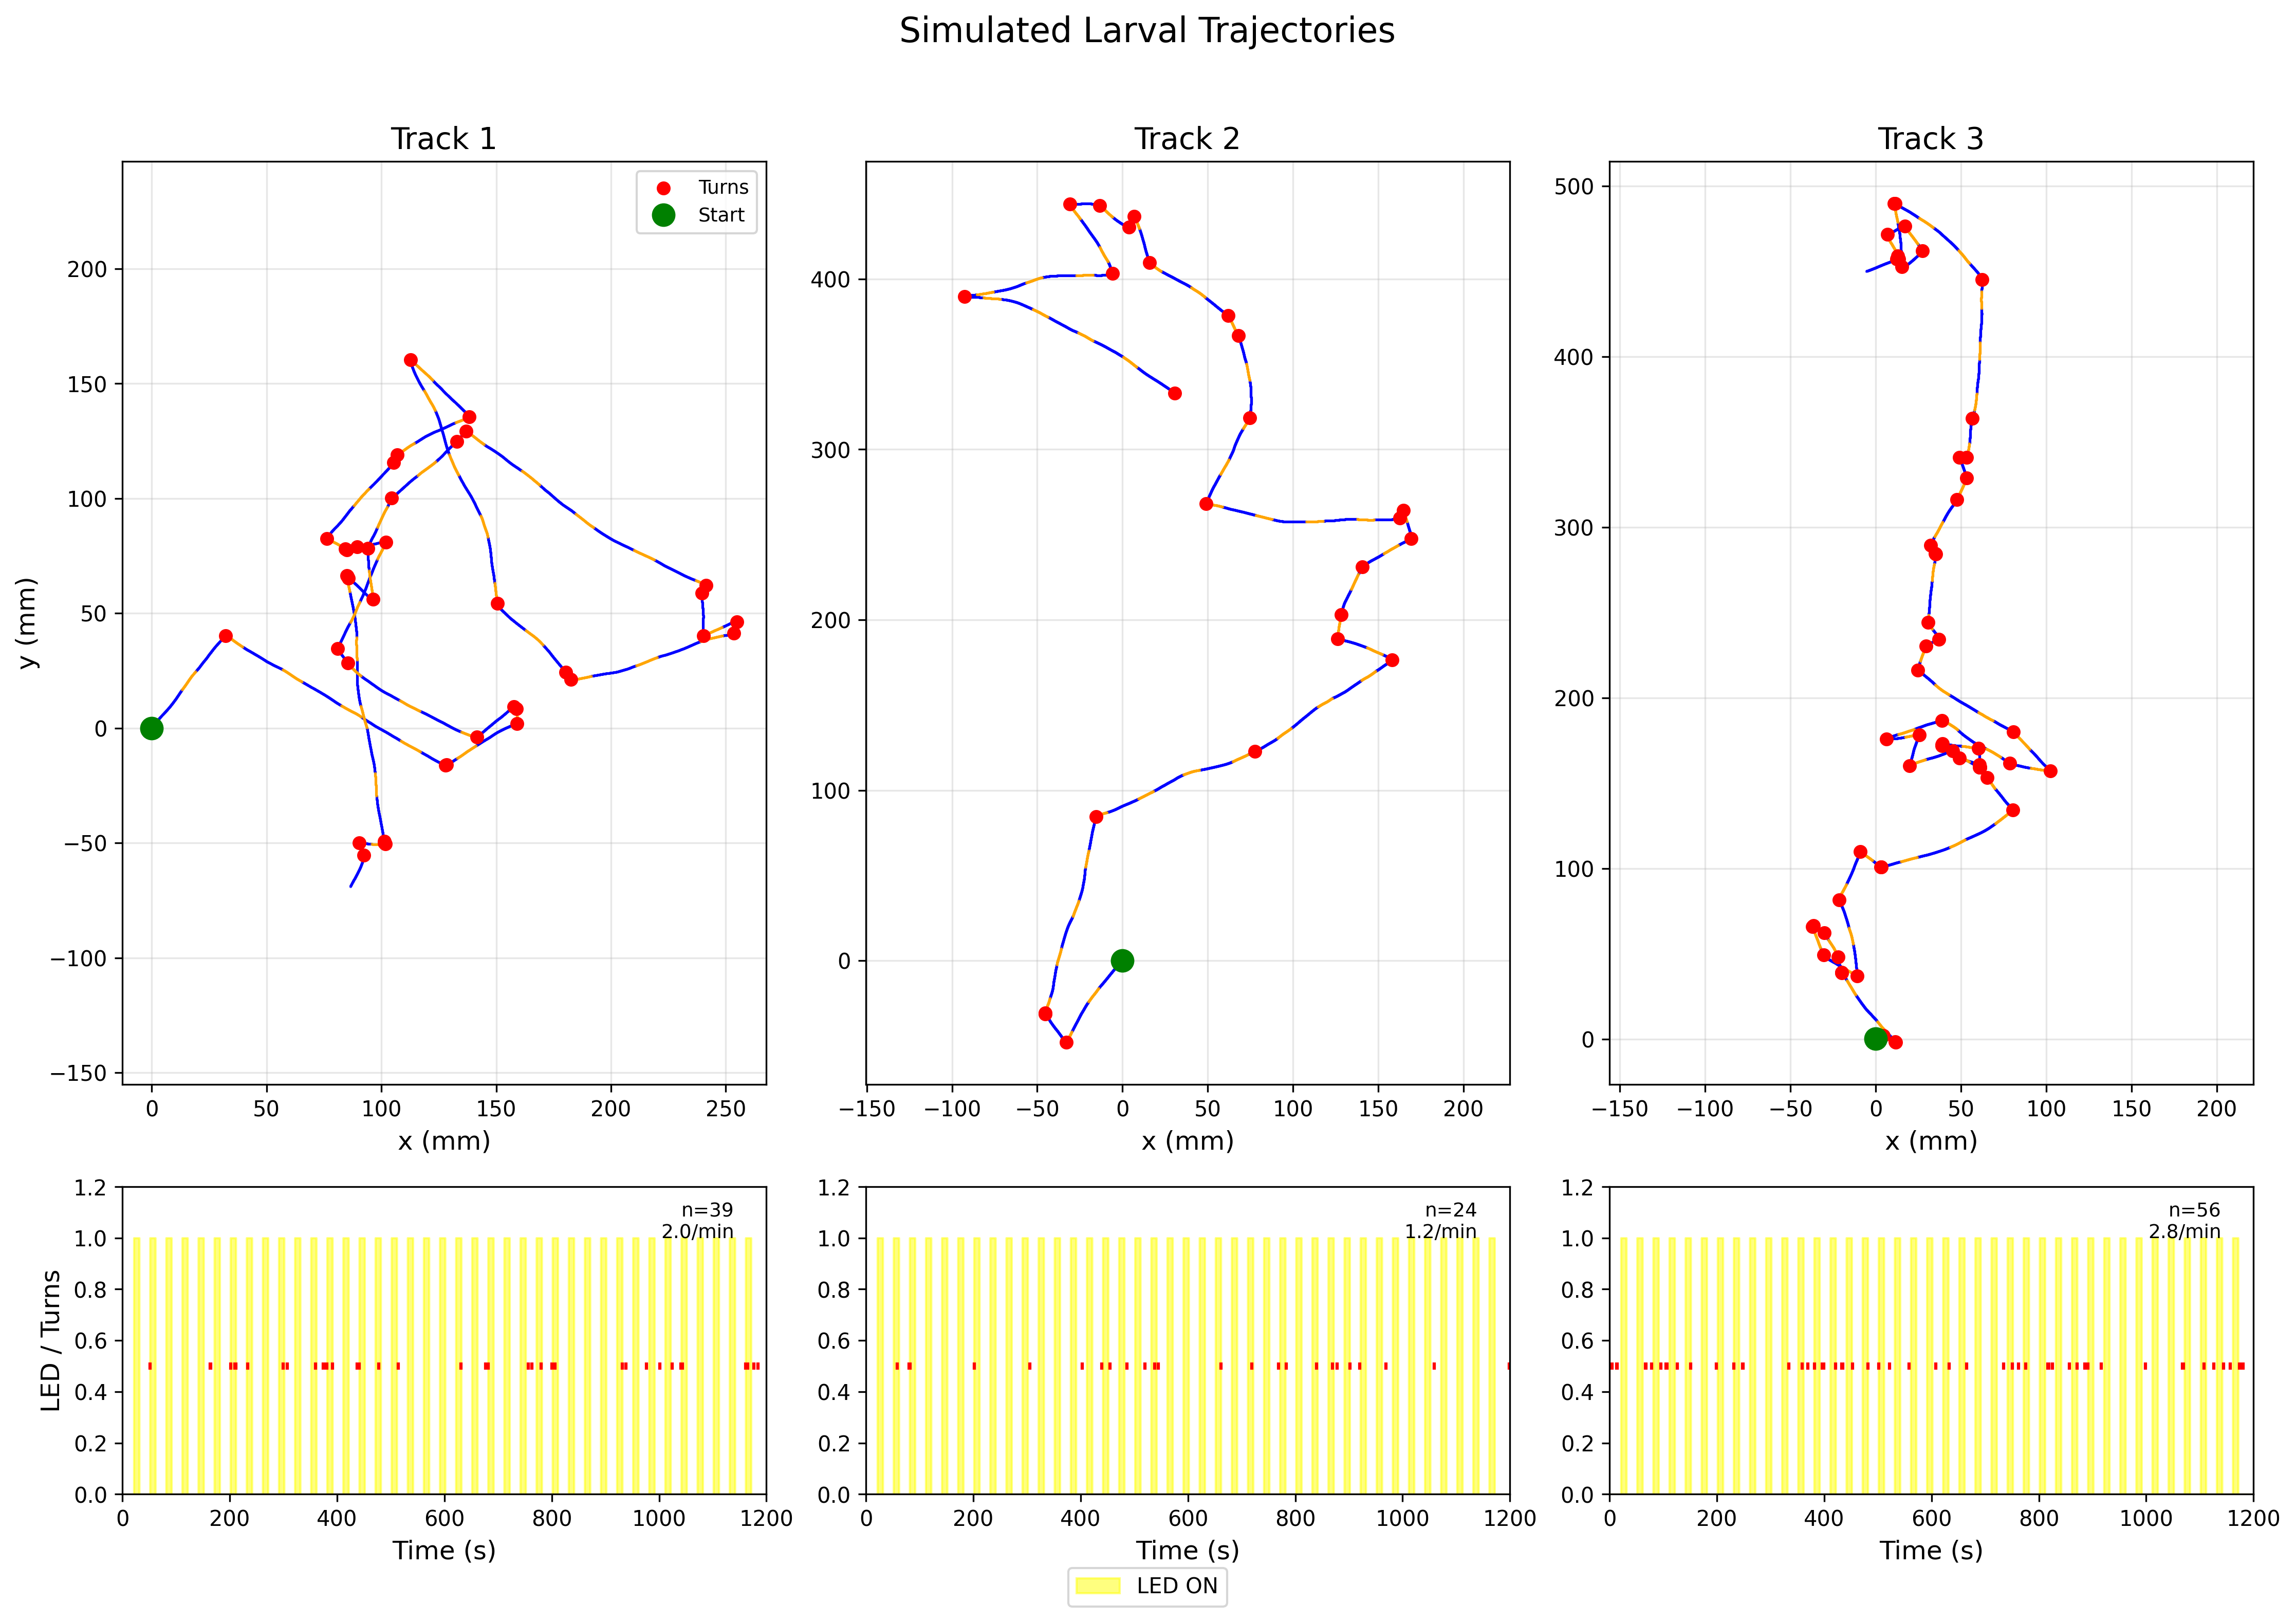
\includegraphics[width=0.95\textwidth]{figure3_trajectories.png}
\caption{\textbf{Trajectory simulation driven by the hazard model.} The RUN/TURN state machine produces realistic larval navigation patterns. \textbf{(A)} Example simulated trajectories (N=5) over 5 minutes, showing characteristic pattern of extended forward runs punctuated by discrete reorientation events. Blue segments indicate RUN state; red circles mark TURN events where heading changes occur. Yellow background shading indicates LED-ON periods (10 s), during which turns are suppressed and runs extend longer. \textbf{(B)} Trajectory detail showing spatial displacement during RUN (forward at 1.0 mm/s with Brownian heading noise, $\sigma = 0.03$ rad/$\sqrt{s}$) and instantaneous heading change during TURN. Turn angles are sampled from $\mathcal{N}(\mu = 7^\circ, \sigma = 86^\circ)$. \textbf{(C)} Turn rate comparison: simulated trajectories produce 1.88 turns/min, closely matching empirical rate of 1.84 turns/min (98\% agreement). The hazard model correctly predicts both the overall event rate and its modulation by LED state.}
\label{fig:trajectories}
\end{figure}

\begin{figure}[htbp]
\centering
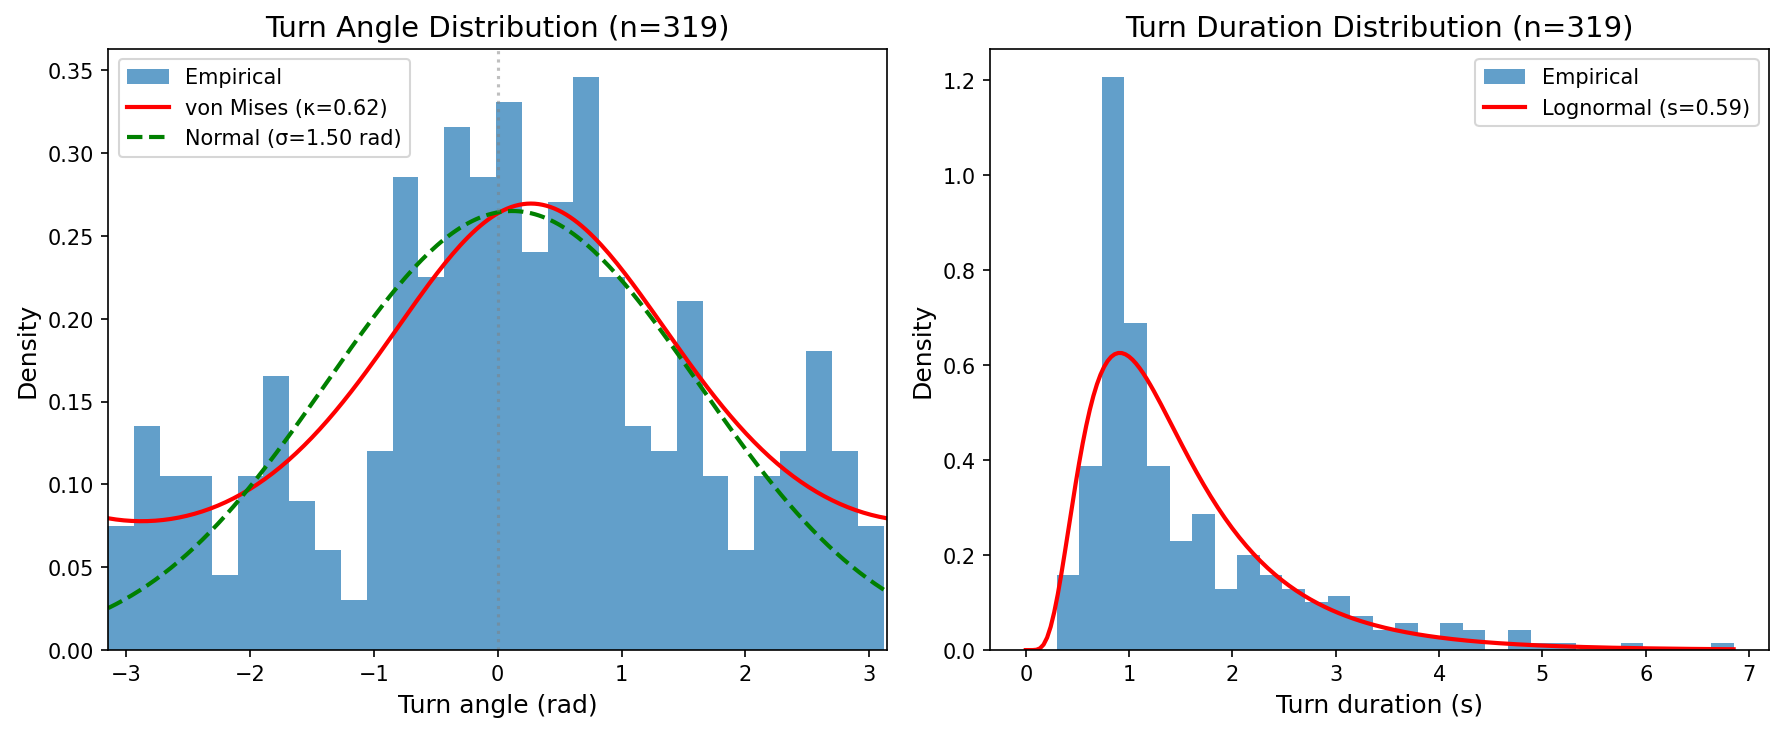
\includegraphics[width=0.95\textwidth]{turn_distributions.png}
\caption{\textbf{Empirical turn angle and duration distributions.} Parameters extracted from 319 filtered events (turn duration $> 0.1$ s) used to parameterize the trajectory simulator. \textbf{(A)} Turn angle distribution: heading changes show high variability with slight rightward bias. A normal distribution (red curve; $\mu = 7^\circ$, $\sigma = 86^\circ$) provides adequate fit. The mean absolute turn angle is $69^\circ$, indicating substantial heading changes during reorientation. The small positive bias may reflect asymmetry in the experimental setup or intrinsic larval handedness. \textbf{(B)} Turn duration distribution: event durations follow a lognormal distribution (red curve; shape $s = 0.59$, scale $= 1.29$ s, median = 1.1 s). Durations range from 0.1--6.8 s, with most turns completing within 2 s. Gamma and exponential fits (not shown) provided poorer fits to the right tail. These distributions enable realistic stochastic simulation of turn kinematics without assuming fixed duration or angle.}
\label{fig:distributions}
\end{figure}

\begin{figure}[htbp]
\centering
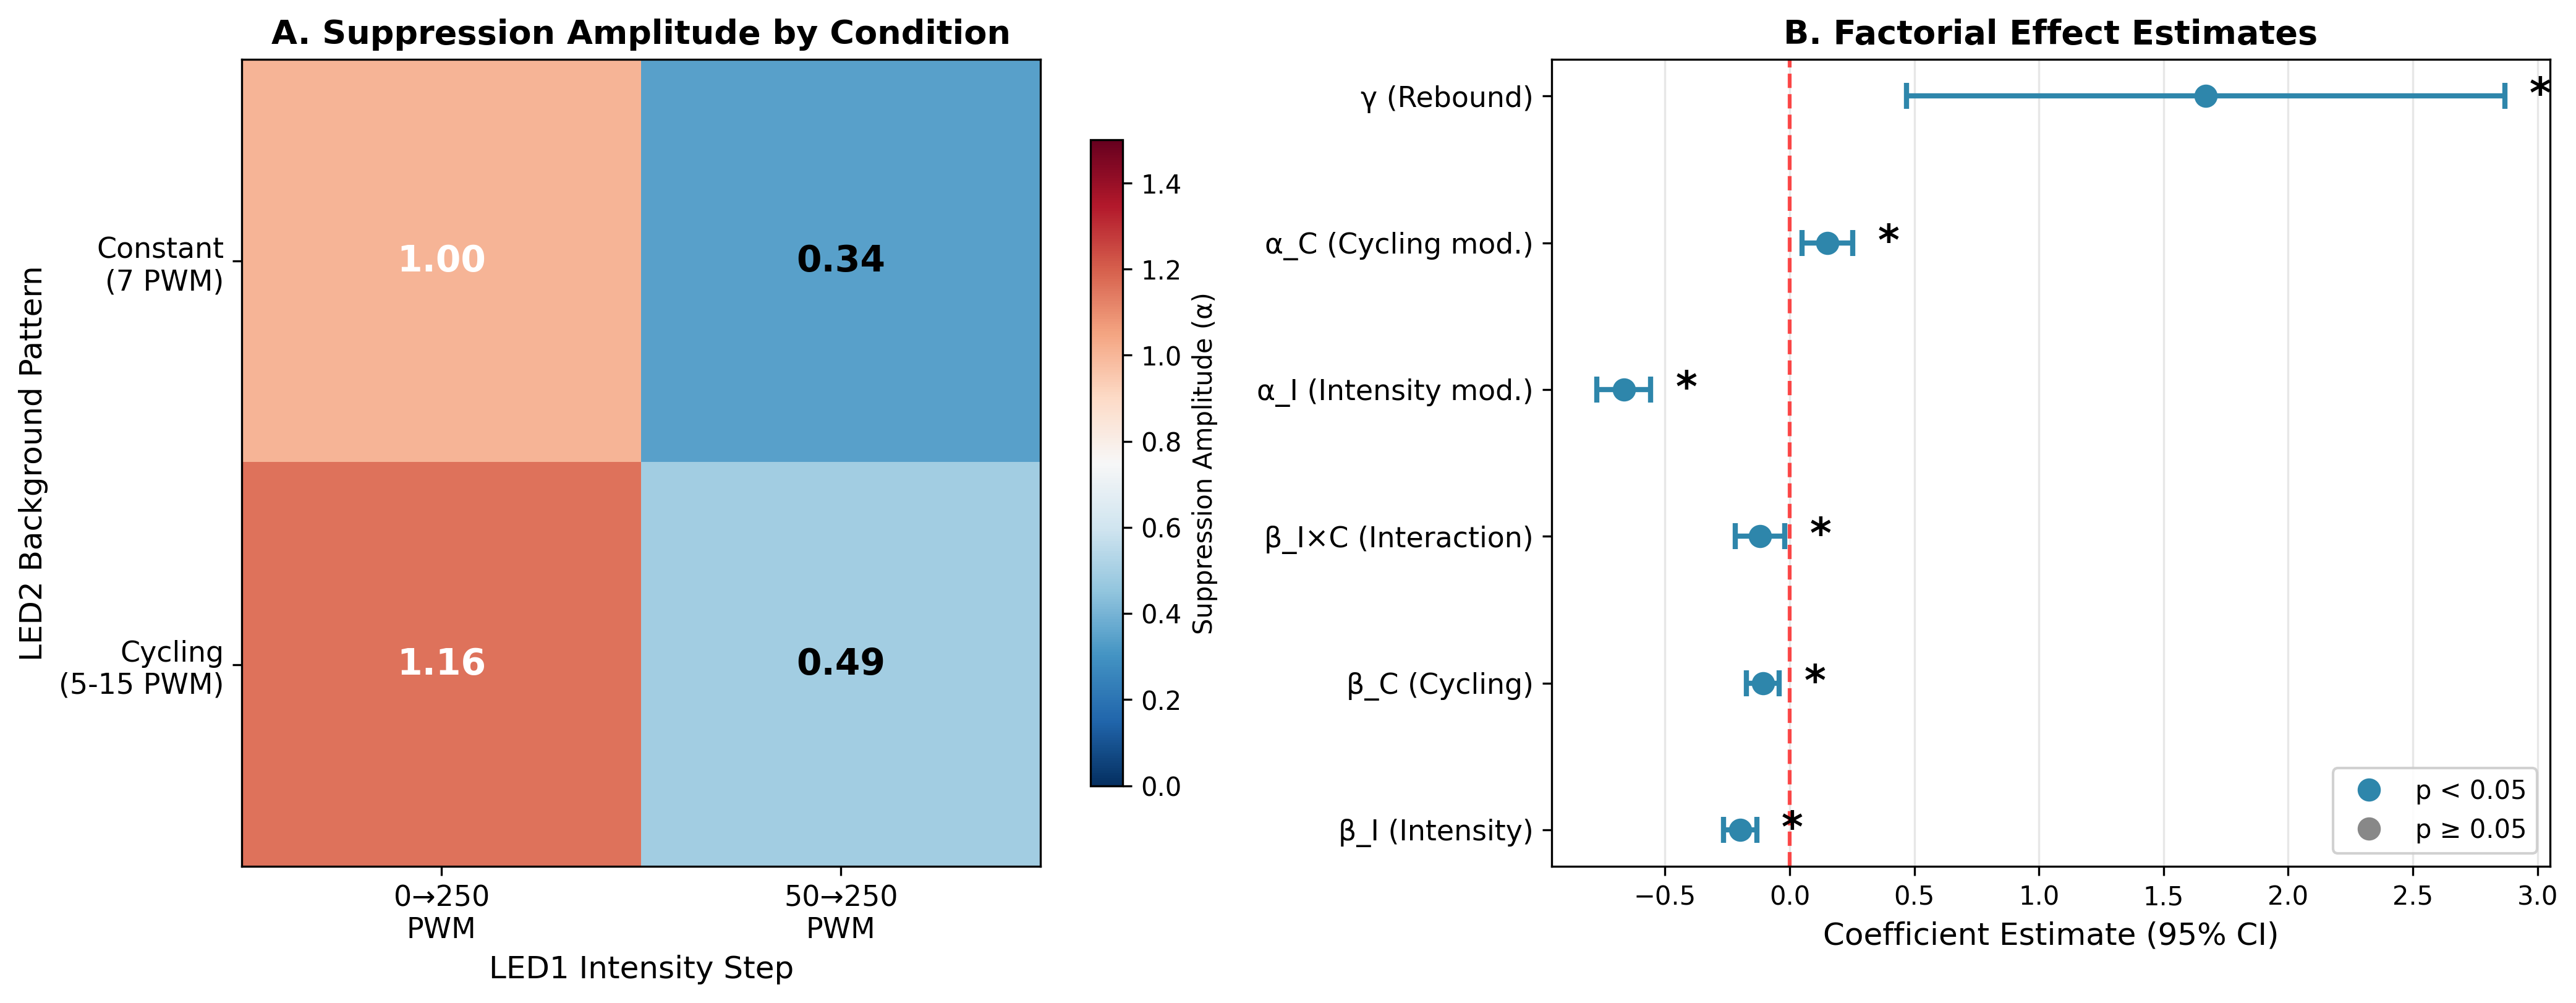
\includegraphics[width=0.95\textwidth]{figure5_factorial.png}
\caption{\textbf{Factorial analysis of intensity and background effects.} Extension of the hazard model to a 2$\times$2 factorial design (12 experiments, 623 tracks, 7,288 events) reveals condition-specific modulation of suppression amplitude. \textbf{(A)} Heatmap of suppression amplitude ($\alpha + \alpha_I \cdot I + \alpha_C \cdot C$) across the four experimental conditions. Values range from 0.34 (50$\rightarrow$250 | Constant, weakest suppression) to 1.16 (0$\rightarrow$250 | Cycling, strongest suppression), representing a 3.4-fold range. Rows: background pattern (Constant 7 PWM vs Cycling 5--15 PWM); columns: LED1 intensity step (0$\rightarrow$250 vs 50$\rightarrow$250 PWM). Blue indicates weaker suppression; red indicates stronger suppression. \textbf{(B)} Forest plot of factorial coefficient estimates with 95\% confidence intervals. All effects are statistically significant ($p < 0.05$, marked with asterisks). Key findings: (1) Intensity modulation ($\alpha_I = -0.665$) indicates 66\% weaker suppression for the 50$\rightarrow$250 condition, consistent with partial adaptation to baseline illumination. (2) Cycling background modulation ($\alpha_C = +0.152$) indicates 15\% stronger suppression with oscillating LED2, suggesting reduced adaptation. (3) The baseline effects ($\beta_I = -0.199$, $\beta_C = -0.108$) show 18\% and 10\% reduction in overall hazard respectively. (4) A synergistic interaction ($\beta_{IC} = -0.119$) indicates greater-than-additive effects when both manipulations are combined. The rebound coefficient ($\gamma = 1.67$) is robustly positive, confirming enhanced event probability after LED offset.}
\label{fig:factorial}
\end{figure}




\end{document}
